\documentclass[a4paper,10pt]{article}
\usepackage[utf8]{inputenc}
\usepackage{polski}
\usepackage{graphicx}
\usepackage{listings}
\usepackage[usenames,dvipsnames]{color}
\addtolength{\hoffset}{-1cm}
\addtolength{\voffset}{-2cm}
\addtolength{\textwidth}{2cm}
\addtolength{\textheight}{3cm}
\usepackage{setspace}
\usepackage{indentfirst}
\usepackage{graphicx}

\lstset{
    language=Matlab,
    basicstyle=\scriptsize,
    aboveskip={1.5\baselineskip},
    columns=fixed,
    showstringspaces=false,
    extendedchars=true,
    breaklines=true,
    tabsize=4,
    prebreak = \raisebox{0ex}[0ex][0ex]{\ensuremath{\hookleftarrow}},
    frame=single,
    showtabs=false,
    showspaces=false,
    showstringspaces=false,
    identifierstyle=\ttfamily,
    keywordstyle=\color[rgb]{0,0,1},
    commentstyle=\color[rgb]{0.133,0.545,0.133},
    stringstyle=\color[rgb]{0.627,0.126,0.941},
    numbers=left,
    numberstyle=\tiny,
    stepnumber=1,
    numbersep=5pt,
    captionpos=b,
    escapeinside={\%*}{*)}
}

\def\figurename{Rys.}
\def\lstlistingname{Fun.}

\title{Informatyczne Systemy Sterowania \\ \large Ćwiczenie 2: Systemy regulacji - Regulator PID}

\author{Adam Jordanek 168139, Tomasz Klimek 168092}

\begin{document}
\maketitle

\section{Wstęp}\label{sec:wstęp}
\subsection{Cel ćwiczenia}
Celem tego ćwiczenia jest poznanie podstawowej struktury systemu sterowania z typową formą algorytmu regulacji PID, oraz zapoznanie się z częścią pakietu M\small ATLAB \normalsize - Simulinkiem, oraz jego możliwości w zakresie modelowania i analizy systemów regulacji.
%Więcej?

\subsection{Plan badań} 
\begin{enumerate}
	\item Symulacja systemu regulacji
	\begin{enumerate}
		\item Regulator P. Zbadać wpływ wartości wzmocnienia regulatora na działanie systemu. 
	    \item Regulator   PI.   Zbadać  wpływ   wartości   parametru   całkowania   na   działanie   systemu 
       (dla ustalonej wartości parametru $k$). 
    	\item Regulator PID. Zbadać wpływ wartości parametru różniczkowania na działanie 
       systemu (dla ustalonych wartości parametrów $k$ i $T_i$). 
	\end{enumerate}
	\item Dobór optymalnych parametrów regulatora. Sporządzenie wykresów:
	\begin{enumerate}
		\item dla regulatora P. 
    	\item dla regulatora PI przy trzech różnych ustalonych wartościach parametru $k$.  
    	\item dla regulatora PID przy trzech różnych wartościach parametru oraz ustalonej wartości parametru $k$.
	\end{enumerate}
	\item Dobór parametrów regulatora PID według zasad Zieglera–Nicholsa
	\begin{enumerate}
		\item Doświadczalnie znaleźć współczynnik wzmocnienia, dla którego układ traci stabilność.
		\item Ustalić okres oscylacji i wzmocnienie krytyczne.
		\item Według odpowiednich rekomendacji określić wartości parametrów regulatora PID.
	\end{enumerate}
\end{enumerate}
Zadania należy wykonać dla obiektu o podanej transmitancji operatorowej:
\begin{equation} \label{eqn:transOS}
G(s) = \frac{b}{s^3 + a_2 s^2 + a_1 s + a_0}
\end{equation}
%Copy/Paste z treści zadania...

\newpage
\section{Realizacja planu i wyniki}

%---------------------------------------------------------------------------------------------------------------------
%
%ZADANIE 1
%
%---------------------------------------------------------------------------------------------------------------------
\subsection{Symulacja systemu regulacji.}\label{sec:zad1}
System regulacji będziemy symulować przy użyciu programu Simulink będącego częścią pakietu M\small ATLAB. \\
\normalsize Schemat systemu służącego nam do symulacji przedstawiony został na poniższym rysunku.

\begin{figure}[h]
    \centering
	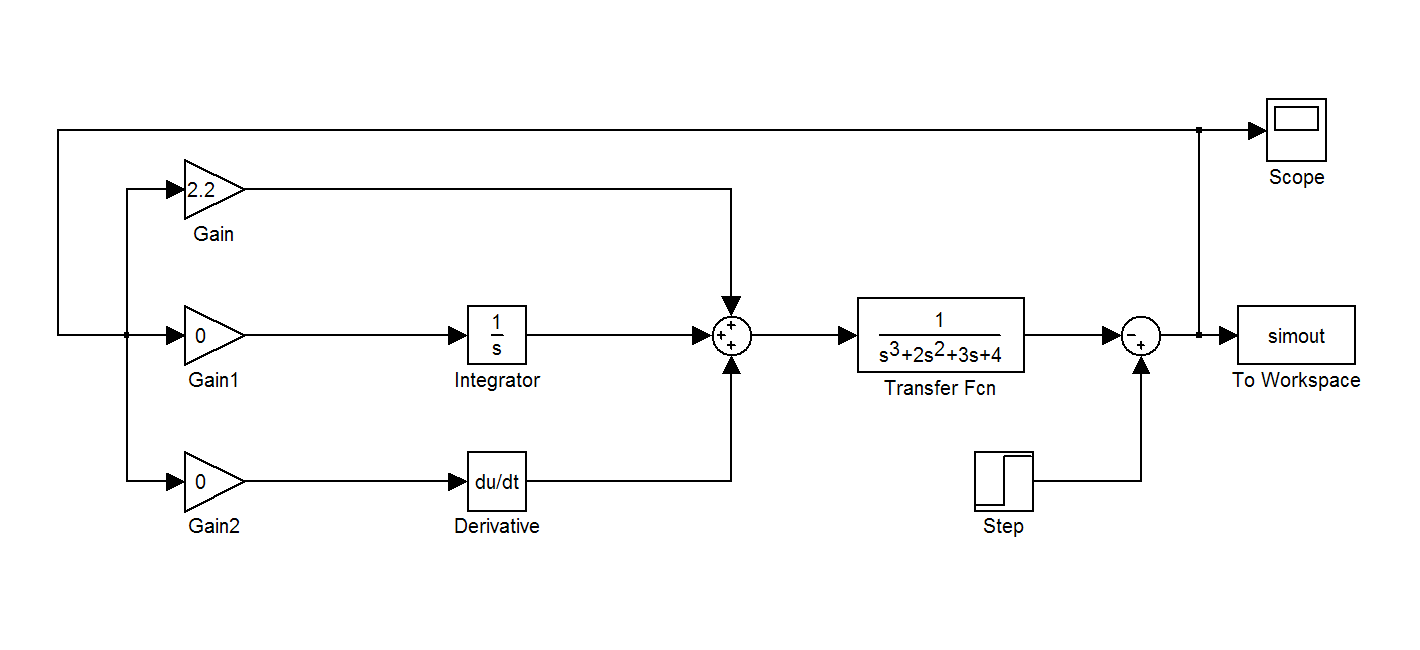
\includegraphics[width=120mm]{CW2-schemat.png}
	\caption{Schemat symulacji obiektu z regulatorem PID}
    \label{fig:Rysunek}
\end{figure}

Wartości błędu regulacji $\varepsilon(t)$ mogą być odczytywane zarówno na wykresie $Scope$ jak i z poziomu M\small ATLABA \normalsize dzięki obiektowi $simout$.

Regulator PID jest opisany następującą transmitancją:
\begin{equation} \label{eqn:transPID}
G(s) = k + {T_{i} \over s} + T_{d}s ,
\end{equation}
gdzie $k$ to współczynnik wzmocnienia, $T_{i}$ to parametr członu całkującego, a $T_{d}$ to parametr członu różniczkującego.

Podczas ćwiczenia przyjęliśmy następujące wartości parametrów transmitancji obiektu sterowania (\ref{eqn:transOS}): 
\begin{equation} \label{eqn:paramTransOS}
b = 1,
a_{2} = 2, 
a_{1} = 3, 
a_{0} = 4
\end{equation}
oraz zadanej wartości wyjścia $y^{*} = 1$.

\subsubsection{Regulator P.}
Aby zasymulować regulator P musieliśmy ustawić wartości parametru całkującego i różniczkującego na $T_{i}=0$, $T_{d}=0$. \\
Następnie wykorzystując poniższą funkcję przetestowaliśmy zachowanie regulatora P dla różnych wartości parametru $k$.
\begin{lstlisting}[caption=Funkcja testująca regulator P.]
function testP(start, step, stop)
load_system('model.mdl');
hold on;
k = start;
i = 0;
color = char('r', 'k', 'b', 'g', 'y', 'm');
set_param('model/Gain1', 'Gain', num2str(0));
set_param('model/Gain2', 'Gain', num2str(0));
while (k <= stop)
    set_param('model/Gain', 'Gain', num2str(k));
    sim('model.mdl');
    wy = simout.signals.values;
    figure(1);
    plot(tout, wy, 'Color', color(mod(i,6)+1));
    i = i + 1;
    q(i) = sum(wy.^2)/length(wy);
    ka(i) = k;
    k = k + step;
end
figure(2);
plot(ka, q);
end
\end{lstlisting}
W ten sposób otrzymalismy następujące wykresy:
\begin{figure}[!h]
    \centering
	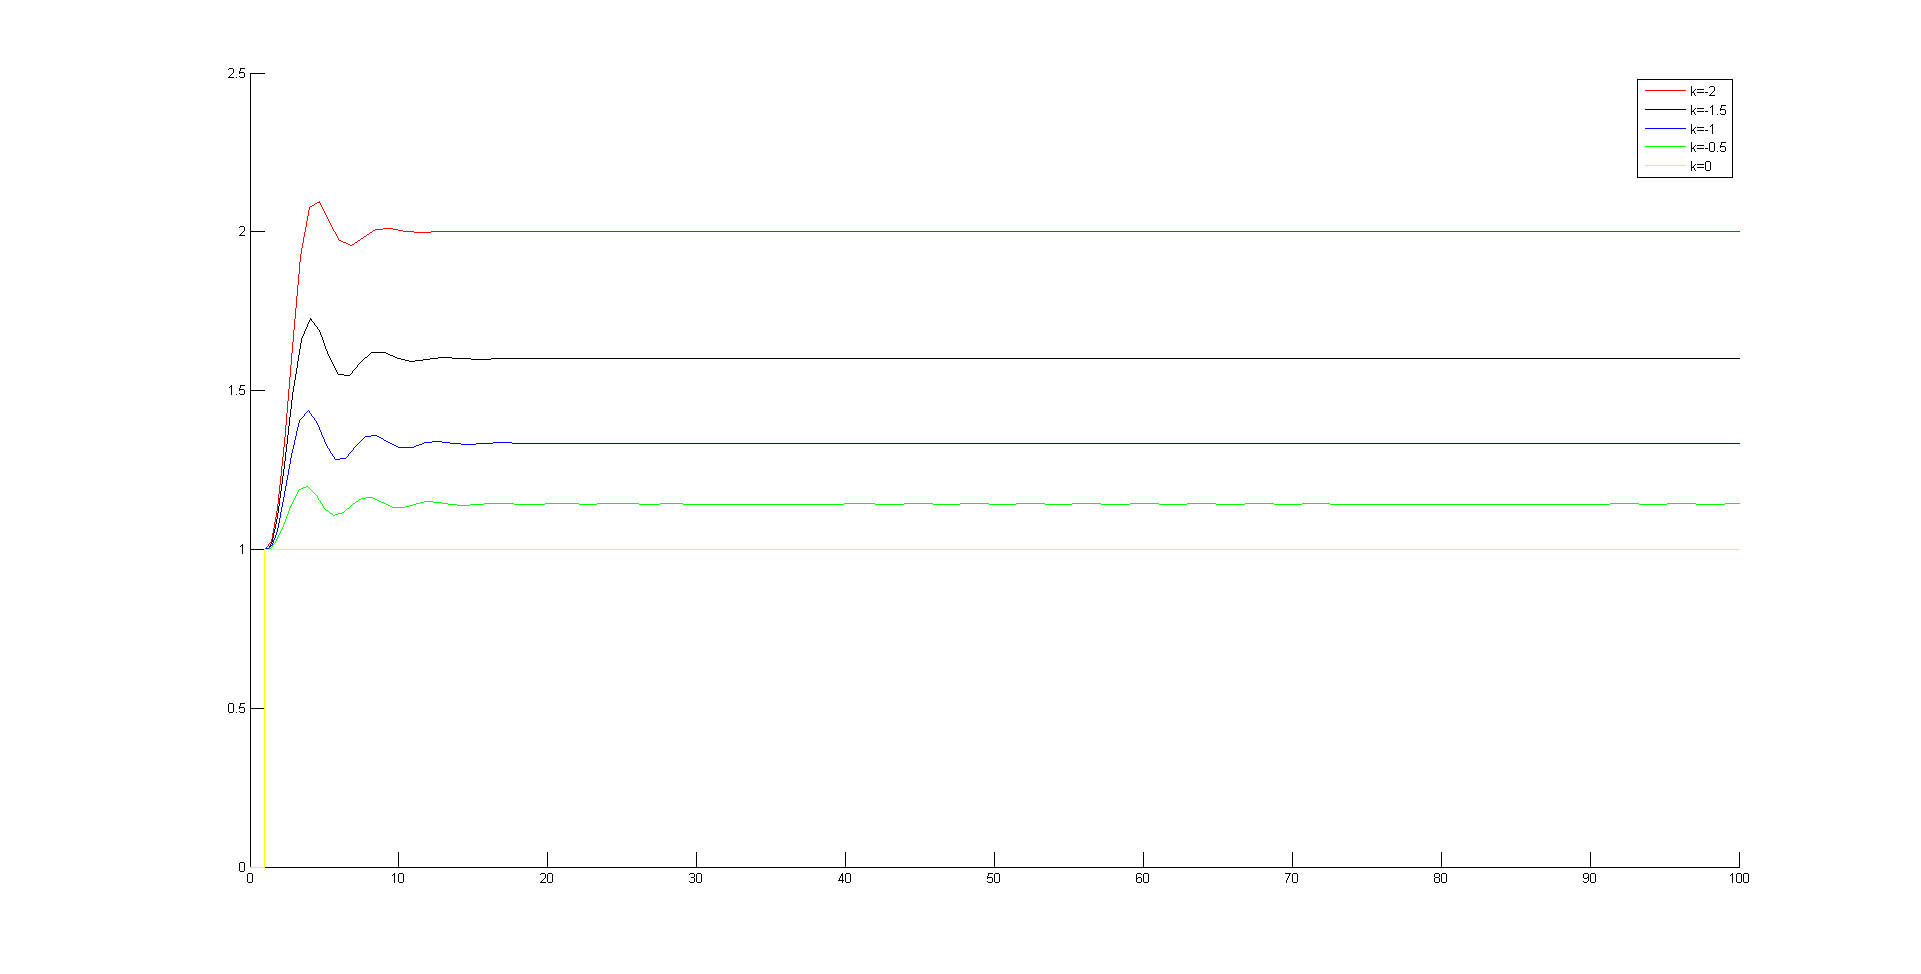
\includegraphics[width=120mm]{CW2-regulatorP-eu.png}
	\caption{Wykres przebiegu funkcji $\varepsilon(t)$ regulatora P dla wartości ujemnych k.}
    \label{fig:regulatorPeu}
\end{figure}
\begin{figure}[!h]
    \centering
	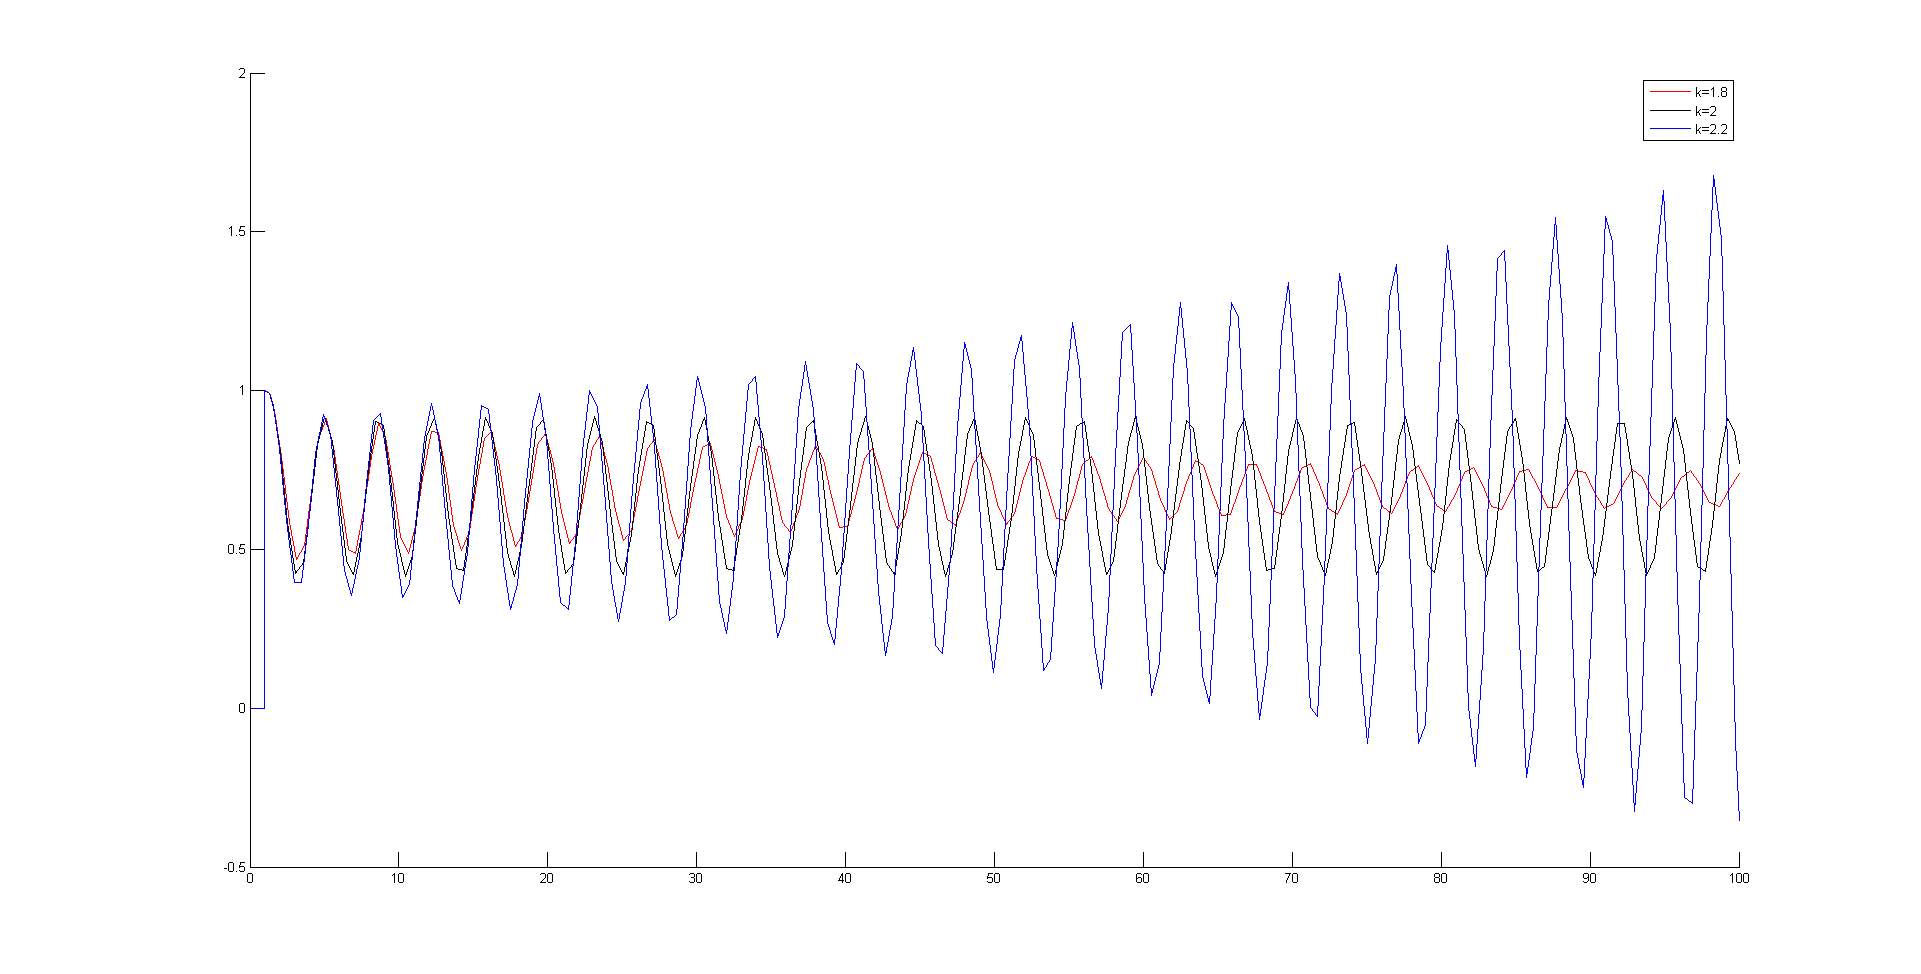
\includegraphics[width=120mm]{CW2-regulatorP-ed.png}
	\caption{Wykres przebiegu funkcji $\varepsilon(t)$ regulatora P dla wartości dodatnich k.}
    \label{fig:regulatorPed}
\end{figure}
%TODO
\subsubsection{Regulator PI.}
Aby zasymulować regulator PI musieliśmy ustawić wartości parametru proporcjonalnego i różniczkującego na $k=2$, $T_{d}=0$. \\
Następnie wykorzystując poniższą funkcję przetestowaliśmy zachowanie regulatora PI dla różnych wartości parametru $T_{i}=0$.
\begin{lstlisting}[caption=Funkcja testująca regulator PI.]
function testPI(start, step, stop)
load_system('model.mdl');
hold on;
ti = start;
i = 0;
color = char('r', 'k', 'b', 'g', 'y', 'm');
set_param('model/Gain', 'Gain', num2str(2));
set_param('model/Gain2', 'Gain', num2str(0));
while (ti <= stop)
    set_param('model/Gain1', 'Gain', num2str(ti));
    sim('model.mdl');
    wy = simout.signals.values;
    figure(1);
    plot(tout, wy, 'Color', color(mod(i,6)+1));
    i = i + 1;
    q(i) = sum(wy.^2)/length(wy);
    tei(i) = ti;
    ti = ti + step;
end
figure(2);
plot(tei, q);
end
\end{lstlisting}
W ten sposób otrzymalismy następujące wykresy:
\begin{figure}[!h]
    \centering
	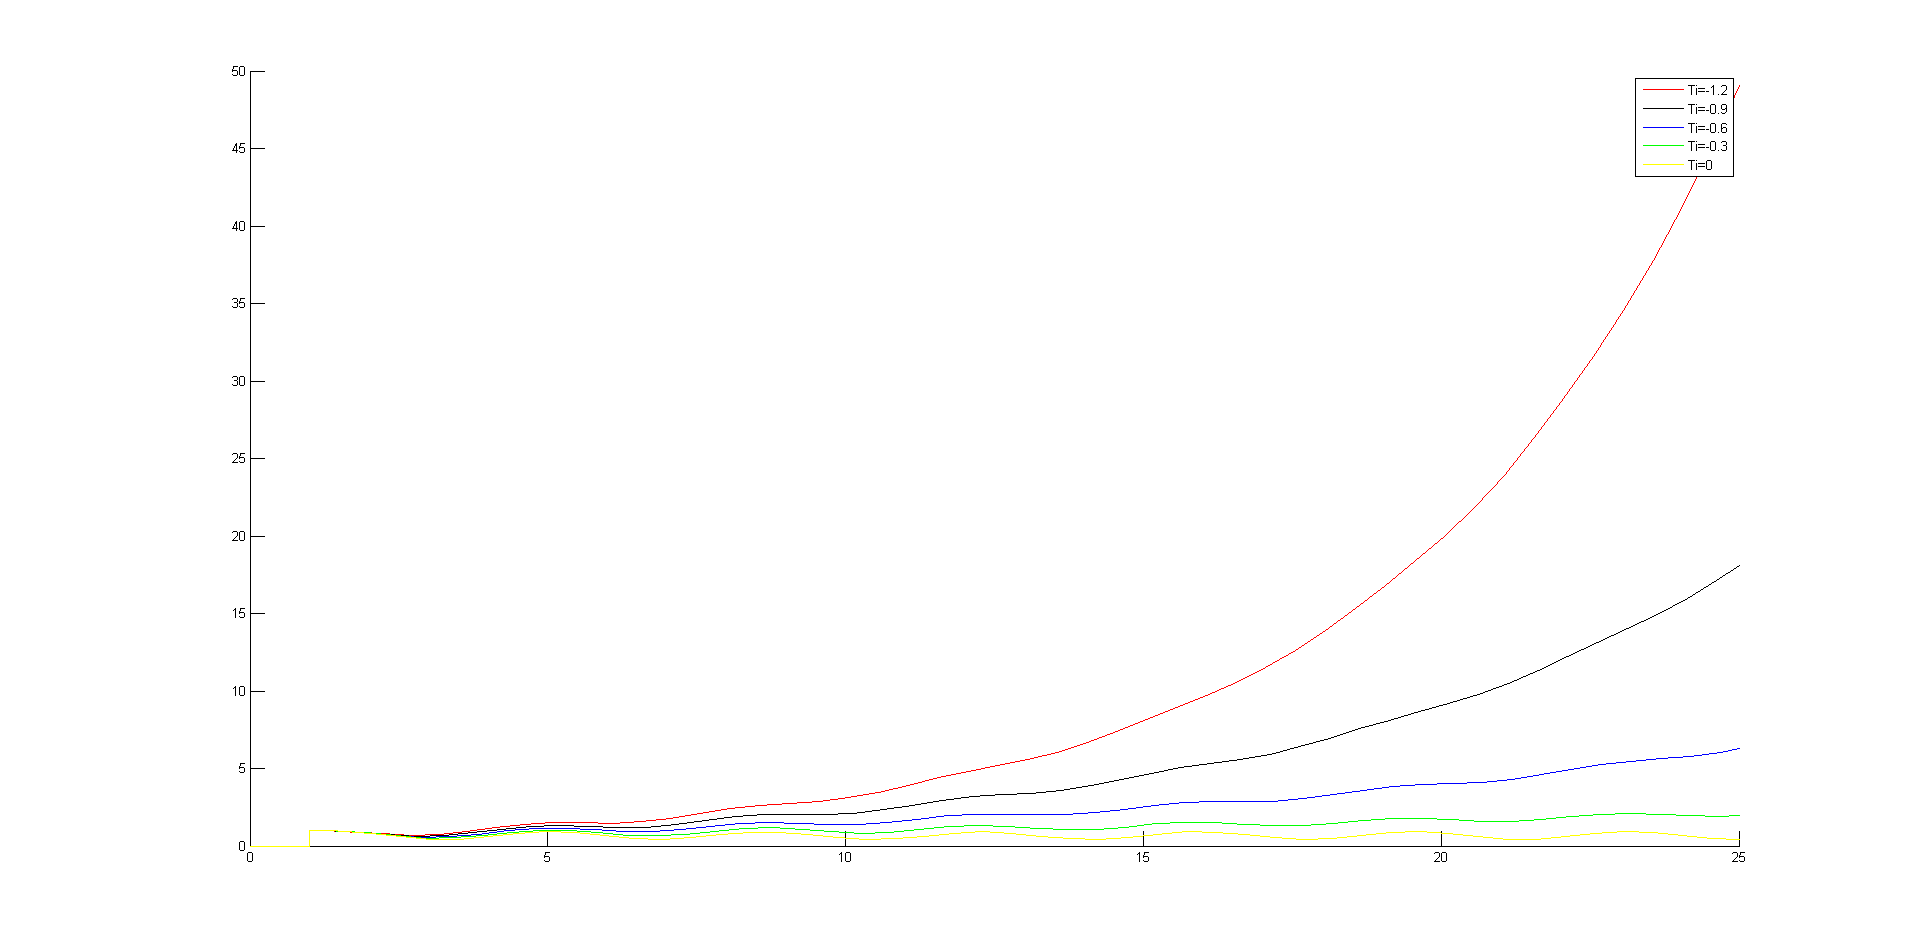
\includegraphics[width=120mm]{CW2-regulatorPI-eu.png}
	\caption{Wykres przebiegu funkcji $\varepsilon(t)$ regulatora P dla wartości ujemnych $T_{i}$.}
    \label{fig:regulatorPeu}
\end{figure}
\begin{figure}[!h]
    \centering
	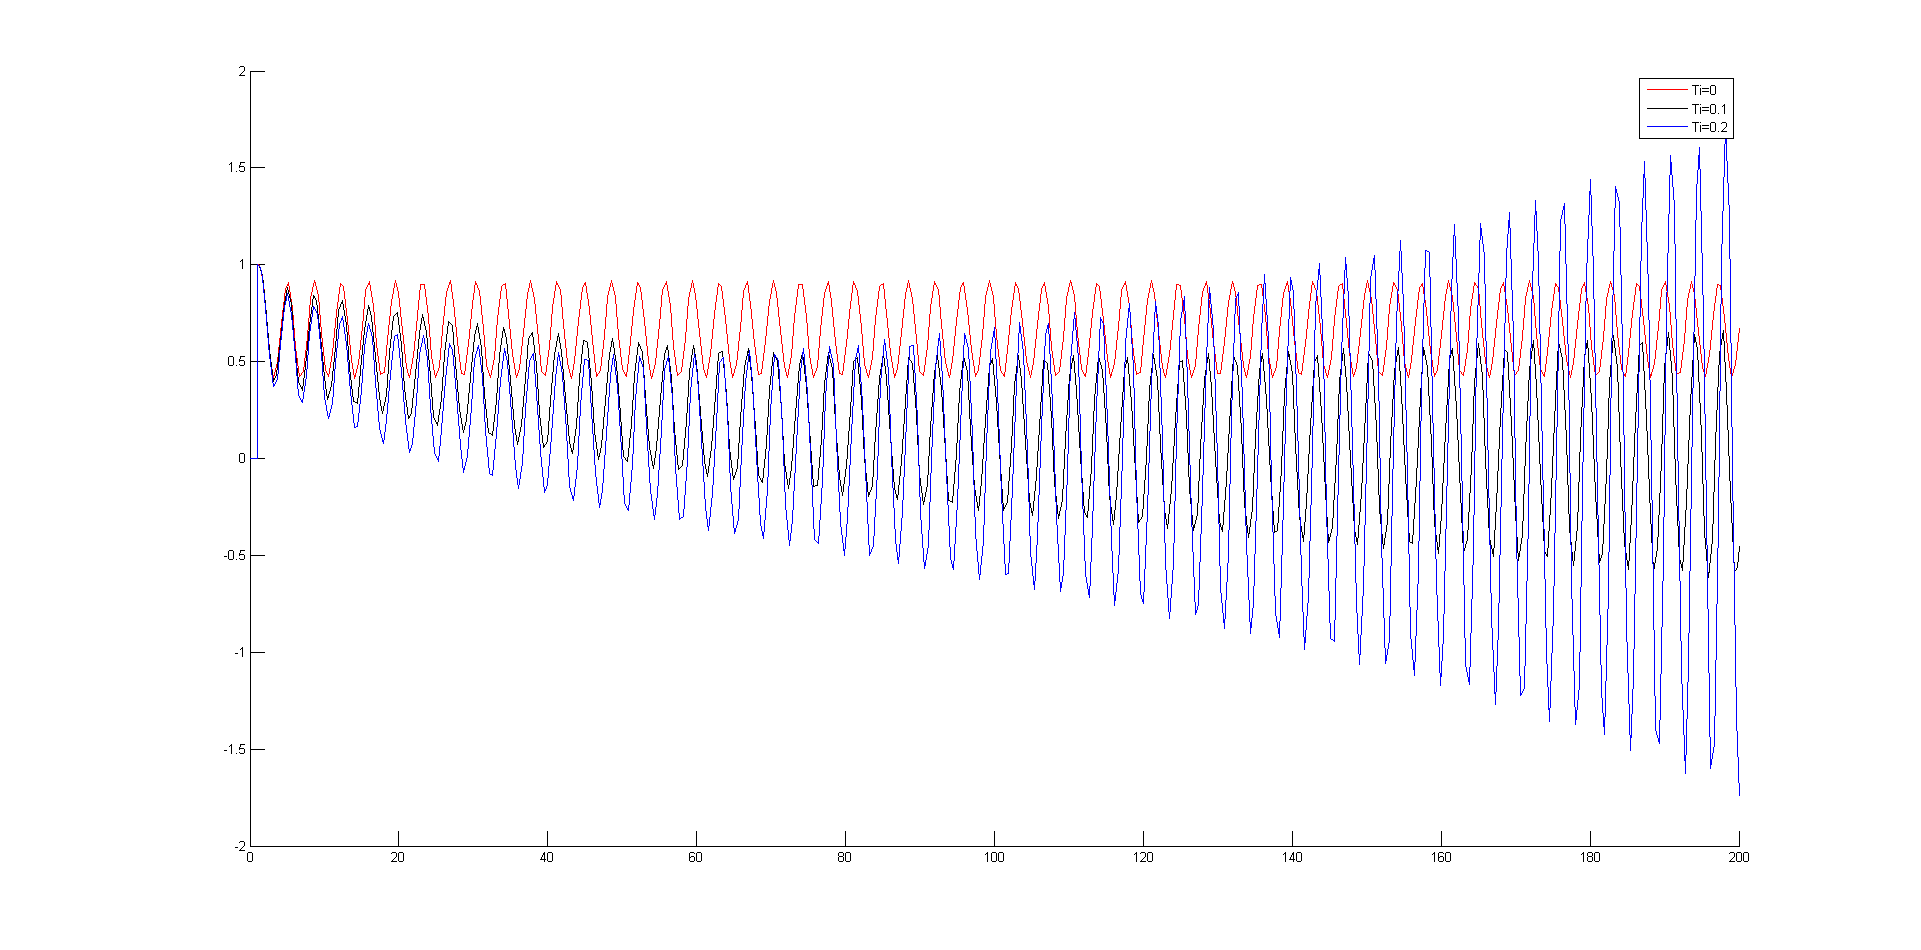
\includegraphics[width=120mm]{CW2-regulatorPI-ed.png}
	\caption{Wykres przebiegu funkcji $\varepsilon(t)$ regulatora P dla wartości dodatnich $T_{i}$.}
    \label{fig:regulatorPed}
\end{figure}
%TODO
\subsubsection{Regulator PID.}
Aby zasymulować regulator P musieliśmy ustawić wartości parametru proporcjonalnego i całkujacego na $k=2$, $T_{i}=1$. \\
Następnie wykorzystując poniższą funkcję przetestowaliśmy zachowanie regulatora P dla różnych wartości parametru $T_{d}$.
\begin{lstlisting}[caption=Funkcja testująca regulator P.]
function testPID(start, step, stop)
load_system('model.mdl');
hold on;
td = start;
i = 0;
color = char('r', 'k', 'b', 'g', 'y', 'm');
set_param('model/Gain', 'Gain', num2str(2));
set_param('model/Gain1', 'Gain', num2str(1));
while (td <= stop)
    set_param('model/Gain2', 'Gain', num2str(td));
    sim('model.mdl');
    wy = simout.signals.values;
    figure(1);
    plot(tout, wy, 'Color', color(mod(i,6)+1));
    i = i + 1;
    q(i) = sum(wy.^2)/length(wy);
    tede(i) = td;
    td = td + step;
end
figure(2);
plot(tede, q);
end
\end{lstlisting}
W ten sposób otrzymalismy następujące wykresy:
\begin{figure}[!h]
    \centering
	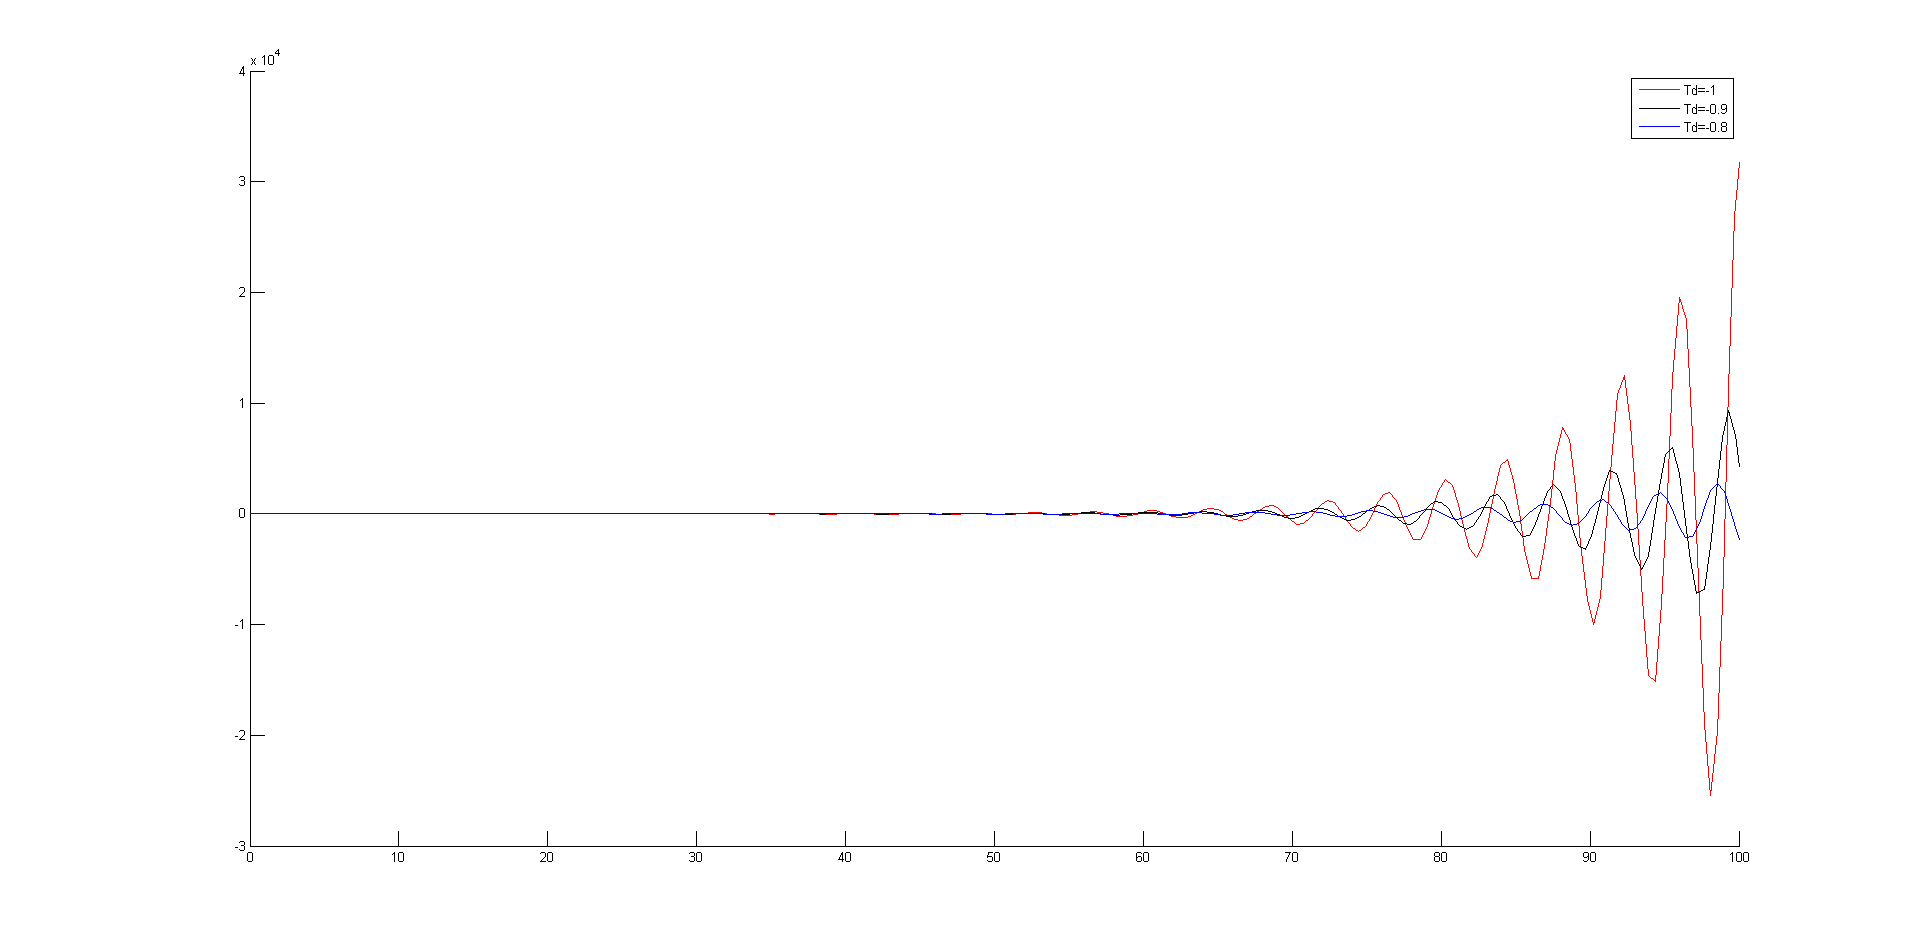
\includegraphics[width=120mm]{CW2-regulatorPID-eu.png}
	\caption{Wykres przebiegu funkcji $\varepsilon(t)$ regulatora P dla wartości ujemnych $T_{d}$.}
    \label{fig:regulatorPeu}
\end{figure}
\begin{figure}[!h]
    \centering
	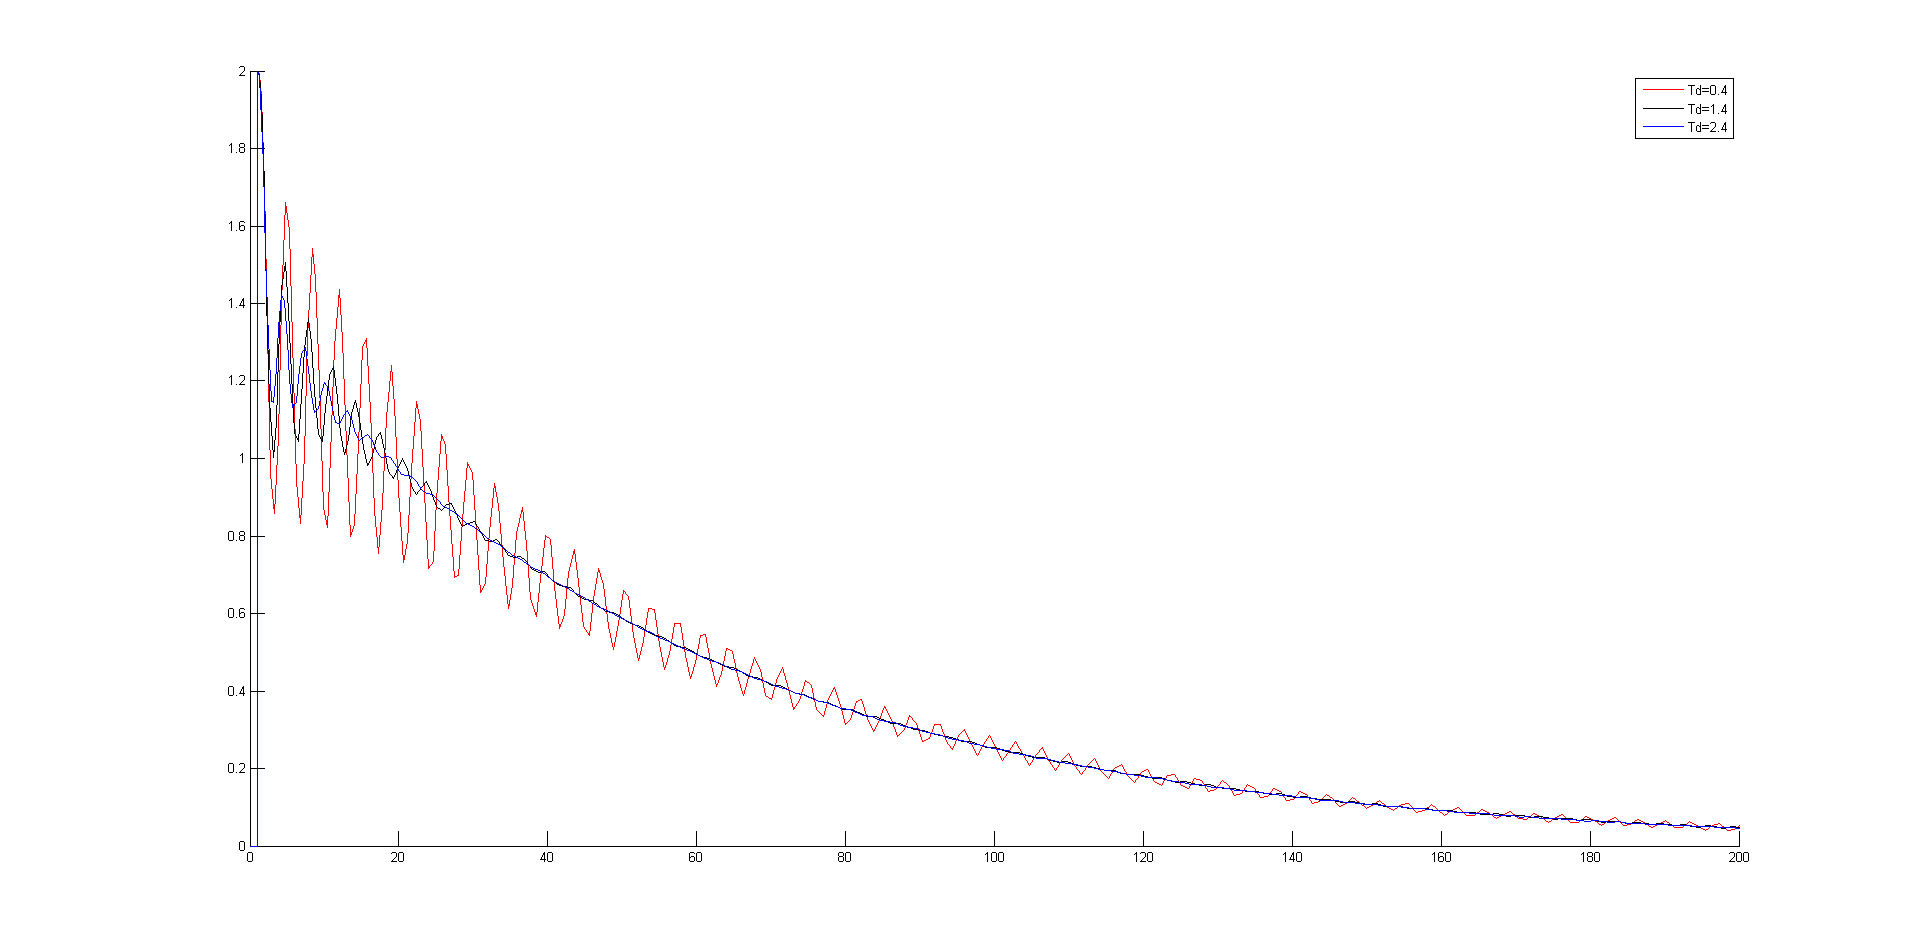
\includegraphics[width=120mm]{CW2-regulatorPID-ed.png}
	\caption{Wykres przebiegu funkcji $\varepsilon(t)$ regulatora P dla wartości dodatnich $T_{d}$.}
    \label{fig:regulatorPed}
\end{figure}
%TODO

\subsection{Dobór optymalnych parametrów regulatora.}\label{sec:zad2}
\subsubsection{Regulator P.}
%TODO
\subsubsection{Regulator PI.}
%TODO
\subsubsection{Regulator PID.}
%TODO
\subsection{Zastosowanie zasad Zieglera-Nicholsa.}\label{sec:zad3}

\section{Wnioski}

\end{document}